\documentclass[10pt]{article}
\usepackage[export]{adjustbox}
\usepackage{amsmath}
\usepackage[makeroom]{cancel}
\usepackage{enumitem}
\usepackage{graphicx}
%Load mhchem using some package options
\usepackage[version=4]{mhchem}
\usepackage{multicol}
\usepackage{siunitx}

\title{
    Problem Set \#7
    \\  \small
    CHEM101A: General College Chemistry
    }
\author{Donald Aingworth IV}
\date{October 23, 2025}

\newcommand{\E}[1]{\times 10^{#1}}
\newcommand{\U}[1]{\underline{#1}}

\begin{document}
    \DeclareSIUnit{\atm}{atm}
    \DeclareSIUnit{\molarity}{M}
    \DeclareSIUnit{\M}{M}

    \maketitle

    \setcounter{section}{7}

    \pagebreak
    \section{Topic D Problem 8}
        Consider the following two facts about the reaction of HCl with NaOH\\
        Fact \#1: $\rm \Delta E$ is a negative number for this reaction, which means that the energy of the chemicals decreases.\\        
        Fact \#2: When HCl and NaOH are mixed, the mixture becomes hotter, which means that the energy of the chemicals increases.
        
        Explain how both of these statements can be true at the same time.

        \subsection{Solution}
            The energy in $\Delta$E referes to the potential energy, not the kinetic energy.
            What likely happened is that the potental energy decreased, so the kinetic energy increased by the potential energy being converted to kinetic energy.

    \pagebreak
    \section{Topic D Problem 9}
        When aqueous HCl reacts with solid \ce{NaHCO3}, the mixture becomes colder.
        \begin{enumerate}[label=\alph*)]
            \item   Does the kinetic energy of the chemicals increase, decrease, or remain the same during the reaction?
            \item   Does the potential energy of the chemical increase, decrease, or remain the same during the reaction?
            \item   What is the sign of $\rm \Delta E$ for this reaction?
        \end{enumerate}
        
        \subsection{Solution (a)}
            The mixture becoming colder implies the temperature decreased, implying the kinetic energy \boxed{\rm decreased}. 
        
        \subsection{Solution (b)}
            The total energy of the system would have to remain the same. 
            Since the kinetic energy decreases, the potential energy must \U{increase}. 

        \subsection{Solution (c)}
            Since $\Delta$E refers to the change in potential energy, the sign of $\Delta$E is \boxed{\rm positive}. 

    \pagebreak
    \section{Topic D Problem 10}
        For the reaction \ce{2 Al(s) + 6 H+(aq) -> 2 Al^3+(aq) + 3 H2(g)}, $\Delta$E = -1057 kJ.
        \begin{enumerate} [label=\alph*)]
            \item   How much energy is given off when 2.822 g of Al reacts with hydrogen ions, assuming the hydrogen ions are in excess?
            \item   How much energy is given off when 1.413 g of Al is added to 23.0 mL of a solution that contains 5.89 M \ce{H+}?
            \item   If you want to obtain 50.0 kJ of energy from this reaction, how many grams of aluminum and how many mL of 3.00 M HCl must you use?
            \item   If this reaction produces 13.3 L of \ce{H2(g)} at 25.0\unit{\celsius} and 1.014 atm, how much energy does it give off?
        \end{enumerate}
        
        \subsection{Solution (a)}
            First convert grams to moles.
            \begin{gather}
                MM(\rm Al)  =   26.98\,\unit{\gram/\mole}\\
                n({\rm Al}) =   \frac{m}{MM}
                    =   \frac{2.822\,\unit{\gram}}{26.98\,\unit{\gram/\mole}}
                    =   0.\U{1045}95997\,\unit{\mole}
            \end{gather}

            Next, we use our favorite ratio for energy.
            \begin{gather}
                \rm
                \frac{\Delta E_{sp}}{n_{sp}(Al)}    =   \frac{\Delta E}{n(Al)}\\
                \frac{\Delta E_{sp}}{0.\U{1045}9\,\unit{\mole}} =   \frac{-1057\,\unit{\kilo\joule}}{2\,\unit{\mole}}
                    =   -\U{528.5}\unit{\kilo\joule/\mole}\\
                \Delta E    =   -\U{55.27}898\,\unit{\kilo\joule}
            \end{gather}

            This means that it releases \boxed{55.28\,\unit{\kilo\joule}}. 

        \subsection{Solution (b)}
            First, find the limiting reactant.
            \begin{align}
                n(\ce{Al})  &=  \frac{m}{MM}
                    =   \frac{1.413\,\unit{\gram}}{26.98\,\unit{\gram/\mole}}
                    =   0.0\U{5231}7\,\unit{\mole}\,\ce{Al}\\
                n(\ce{H+})  &=  cV
                    =   (5.89\,\unit{\mole/\liter}) (23.0\,\unit{\milli\mole})
                    =   0.\U{135}47\,\unit{\mole}\,\ce{H+}
            \end{align}

            Dividing the number of moles of \ce{H+} by 6 and the number of moles of \ce{Al} by 2 makes clear that the \ce{H+} is the limiting reactant.
            From here, just use our favorite ratio again.
            \begin{gather}
                \frac{\Delta E_{sp}}{0.\U{135}47\,\unit{\mole}}    =   \frac{-1057\,\unit{\kilo\joule}}{6\,\unit{\mole}}
                    =   176.167\,\unit{\kilo\joule/\mole}\\
                \Delta E_{sp}   =   \U{23.8}653\,\unit{\kilo\joule}
            \end{gather}

            That means it releases \boxed{23.9\,\unit{\kilo\joule}}. 
        
        \subsection{Solution (c)}
            In this instance, it would have to be that $\Delta E_{sp} = -50.0\unit{\kilo\joule}$. 
            We can put this into our favorite ratio to find the number of necessary moles of each. 
            \begin{gather}
                \frac{-50.0\,\unit{\kilo\joule}}{n(\ce{Al})}    =   \frac{-1057\,\unit{\kilo\joule}}{2\,\unit{\mole}}\\
                n(\ce{Al})  =   \frac{50.0\,\unit{\kilo\joule}}{528.5\,\unit{\kilo\joule/\mole}}
                    =   0.0\U{946}0738\,\unit{\mole}\\
                \frac{-50.0\,\unit{\kilo\joule}}{n(\ce{H+})}    =   \frac{-1057\,\unit{\kilo\joule}}{6\,\unit{\mole}}\\
                n(\ce{H+})  =   \frac{50.0\,\unit{\kilo\joule}}{\U{176.1}667\,\unit{\kilo\joule/\mole}}
                    =   0.\U{283}8221\,\unit{\mole}
                    =   n(\ce{HCl})
            \end{gather}

            Now we can convert both to their requested units.
            \begin{align}
                m(\ce{Al})  &=  n * MM
                    =   0.0\U{946}0738\,\unit{\mole} * 26.98\,\unit{\gram/\mole}\\
                    &=  \boxed{2.55\,\unit{\gram}}\\
                V(\ce{H+})  &=  \frac{n}{M}
                    =   \frac{0.\U{283}8221\,\unit{\mole}}{3.00 \text{ M HCl}}
                    =   \boxed{0.0946\,\unit{\liter}}
            \end{align}

        \subsection{Solution (d)}
            Use the ideal gas law to find the number of moles.
            \begin{align}
                PV  &=  nRT\\
                n   &=  \frac{PV}{RT}
                    =   \frac{(1.014\,\unit{\atm})(13.3\,\unit{\liter})}{(0.08206\,\unit{\atm\cdot\liter/\mole\cdot\kelvin})(298.15\,\unit{\kelvin})}\\
                    &=  0.\U{551}2178\,\unit{\mole}
            \end{align}

            This can be used with our favorite ratio.
            \begin{gather}
                \frac{\Delta E_{sp}}{n_{sp}(\ce{H2})}  =   \frac{\Delta E}{n(\ce{H2})}\\
                \frac{\Delta E_{sp}}{0.\U{551}2178\,\unit{\mole}}  =   \frac{-1057\,\unit{\kilo\joule}}{3\,\unit{\mole}}
                    =   -\U{352}.333\,\unit{\kilo\joule/\mole}\\
                \Delta E_{sp}   =   (0.\U{551}2178\,\unit{\mole}) (-\U{352}.333\,\unit{\kilo\joule/\mole})
                    =   \U{194.2}1\,\unit{\kilo\joule}
                    =   \boxed{194.2\,\unit{\kilo\joule}}
            \end{gather}

    \pagebreak
    \section{Topic D Problem 11}
        When 4.00 g of \ce{Br2} reacts with excess Al to form \ce{AlBr3}, 8.80 kJ of energy is given off.
        Calculate $\Delta E$ for the reaction \ce{2 Al(s) + 3 Br2(s) -> 2 AlBr3(s)}.
        
        \subsection{Solution}
            First convert the number of grams of \ce{Br2} to moles. 
            \begin{align}
                n(\ce{Br2}) &=  \frac{4.00\,\unit{\gram}}{159.8\,\unit{\gram/\mole}}
                    =   0.0\U{250}313\,\unit{\mole}
            \end{align}

            Next, use our favorite fraction.
            \begin{gather}
                \frac{\Delta E}{n(Br2)} =   \frac{\Delta E_{sp}}{n_{sp}(Br2)}\\
                \frac{\Delta E}{3\,\unit{\mole}}    =   \frac{-8.80\,\unit{\kilo\joule}}{0.0\U{250}313\,\unit{\mole}}
                    =   -\U{351}.56\,\unit{\kilo\joule/\mole}\\
                \Delta E    =   (3\,\unit{\mole}) (\U{351}.56\,\unit{\kilo\joule/\mole})
                    =   -\U{105}4.68\,\unit{\kilo\joule}
                    =   \boxed{-1.054\,\unit{\mega\joule}}
            \end{gather}

    \pagebreak
    \section{Topic D Problem 12}
        A chemist burns 0.5177 g of liquid hexane (\ce{C6H14}) in a bomb calorimeter that has a heat capacity of 4287 J/\unit{\celsius}. 
        The temperature of the calorimeter rises from 21.382\unit{\celsius} to 27.170\unit{\celsius} during the reaction. 
        Calculate $\Delta$E for the following reaction: 
        \begin{center}
            \ce{2 C6H14(l) + 19 O2(g) -> 12 CO2(g) + 14 H2O(l)}
        \end{center}
        
        \subsection{Solution}
            \begin{center}
                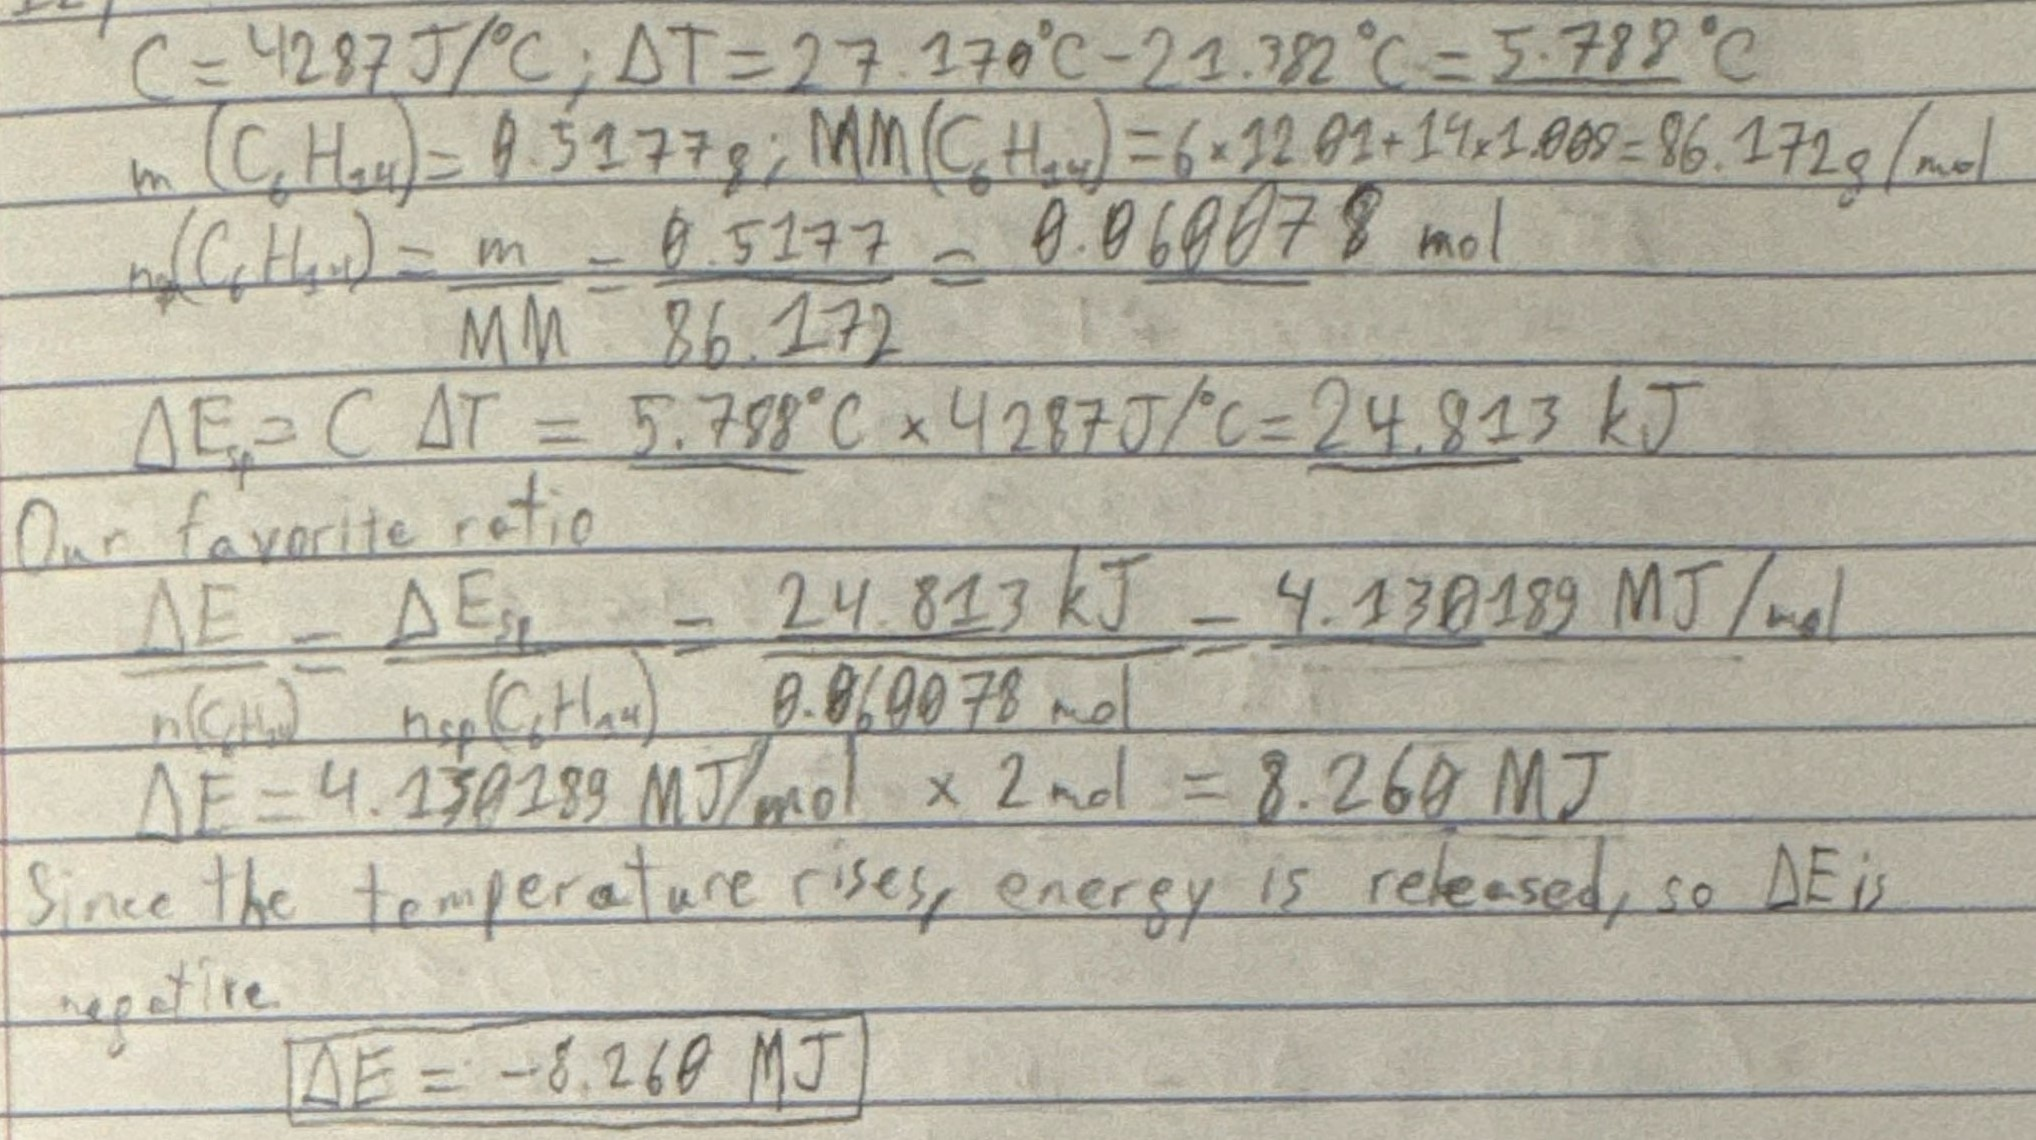
\includegraphics[width=\textwidth]{Answers Images/Problem 12.jpg}
            \end{center}

    \pagebreak
    \section{Topic D Problem 13}
        Explain why some reactions give off different amounts of heat when they are carried out at constant pressure versus constant volume.
        
        \subsection{Solution}
            I just did Thermodynamics in Physics, so that's the perspective I'm approaching this from.
            \begin{equation}
                W   =   P \Delta V
            \end{equation}
            When you carry out a reaction at constant pressure, the volume can still change. 
            This volume change allows work to be done because the work depends on the change in volume but only the raw value of the pressure.
            Meanwhile, when you carry out a reaction at constant volume, no work can be done because the work is dependant on the change in volume, not the raw value. 

    \pagebreak
    \section{Topic D Problem 14}
        A reaction has $\Delta E$ = -50 kJ.
        \begin{enumerate}[label=\alph*)]
            \item   If this reaction occurs, will the reaction mixture become hotter, or colder?
            \item   Is this an exothermic reaction, or is it an endothermic reaction?
            \item   After this reaction has occurred, will the potential energy of the chemical mixture be higher than, lower than, or the same as it was before the reaction?
            \item   After this reaction has occurred, will the kinetic energy of the universe be higher than, lower than, or the same as it was before the reaction (assuming no other reaction has occurred)?
        \end{enumerate}
        
        \subsection{Solution}
            \begin{enumerate}[label=\alph*)]
                \item   Immediately, the mixture will become \U{hotter}, but the temperature will even out to equilibrium over time.
                \item   Since the energy causes the mixture to warm up and exert energy from within, the process would be \U{endothermic}.
                \item   It would be \U{lower}.
                \item   The kinetic energy of the universe will \U{increase}. 
            \end{enumerate}

    \pagebreak
    \section{Topic D Problem 15}
        A reaction has $\Delta E$ = 10 kJ, and it converts a solid into a gas.
        \begin{enumerate}[label=\alph*)]
            \item If this reaction occurs in a closed, rigid container, will the amount of heat that is absorbed be larger than 10 kJ, smaller than 10 kJ, or exactly 10 kJ? Justify your answer.
            \item If this reaction occurs in an open container, will the amount of heat that is absorbed be larger than 10 kJ, smaller than 10 kJ, or exactly 10 kJ? Justify your answer.
            \item Will PV work be done in either part a or part b? If so, which part(s)?
            \item What is the sign of the PV work when PV work occurs?
        \end{enumerate}
        
        \subsection{Solution}

    \pagebreak
    \section{Topic D Problem 16}
        A reaction has $\Delta E$ = -10 kJ, and it converts a gas into a liquid.
a) If this reaction occurs in a closed, rigid container, will the amount of heat that is given off
be larger than 10 kJ, smaller than 10 kJ, or exactly 10 kJ? Justify your answer.
b) If this reaction occurs in an open container, will the amount of heat that is given off be
larger than 10 kJ, smaller than 10 kJ, or exactly 10 kJ? Justify your answer.
c) Will PV work be done in either part a or part b? If so, which part(s)?
d) What is the sign of the PV work when PV work occurs?
        
        \subsection{Solution}

    \pagebreak
    \section{Topic D Problem 17}
        A reaction has $\Delta E$ = -10 kJ, and it converts a liquid into a gas.
a) If this reaction occurs in a closed, rigid container, will the amount of heat that is given off
be larger than 10 kJ, smaller than 10 kJ, or exactly 10 kJ? Justify your answer.
b) If this reaction occurs in an open container, will the amount of heat that is given off be
larger than 10 kJ, smaller than 10 kJ, or exactly 10 kJ? Justify your answer.
c) Will PV work be done in either part a or part b? If so, which part(s)?
d) What is the sign of the PV work when PV work occurs?
        
        \subsection{Solution}

    \pagebreak
    \section{Topic D Problem 18}
        a) What is the PV work when 3.00 moles of liquid water boils at 100\unit{\celsius} at constant pressure? 
        Give your answer in kJ, and include the correct sign.\\
        b) What is the PV work when 3.00 moles of steam condenses at 100\unit{\celsius} at constant pressure?
        Give your answer in kJ, and include the correct sign.

        
        \subsection{Solution}
            \begin{center}
                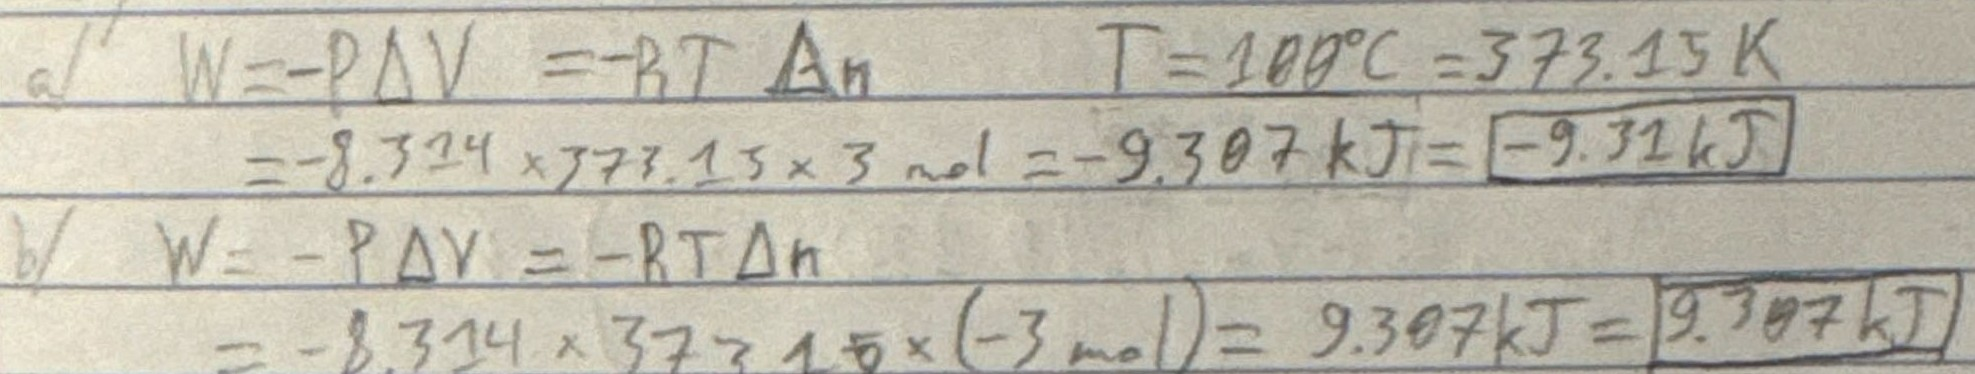
\includegraphics[width=\textwidth]{Answers Images/Problem 18.jpg}
            \end{center}

    \pagebreak
    \section{Topic D Problem 19}
        Consider the following reaction:
        \begin{center}
            \ce{4 C3H9N(l) + 21 O2(g) -> 12 CO2(g) + 18 H2O(l) + 2 N2(g)} $\Delta E$ = -9667 kJ
        \end{center}
        The following questions (parts a through j) refer to this reaction.
        \begin{enumerate}[label=\alph*)]
            \item   Calculate $\Delta H$ for this reaction at 25\unit{\celsius}.
            \item   How much heat will be given off if 8.250 g of \ce{C3H9N} reacts with excess \ce{O2} in a closed, rigid container at 25\unit{\celsius}?
            \item   How much heat will be given off if 8.250g of \ce{C3H9N} reacts with excess \ce{O2} in an open container at 25\unit{\celsius}?
            \item   Calculate the PV work in part b. Include the correct sign.
            \item   Calculate the PV work in part c. Include the correct sign.
            \item   If you want to obtain 200.0 kJ of heat by reacting \ce{C3H9N} with \ce{O2} in an open container, what mass of \ce{C3H9N} must you use?
            \item   How much heat is produced when 2.199 g of liquid \ce{C3H9N} reacts with 5.738 g of gaseous \ce{\ce{O2}} in an open container?
            \item   If you burn enough liquid \ce{C3H9N} to produce 841.2 kJ of heat in an open container, what volume of gaseous N2 will you form at 25.0\unit{\celsius} and 752 torr?
            \item   If this reaction is carried out in a closed, rigid container and produces 31.74 g of liquid \ce{H2O}, how much heat does it produce?
        \end{enumerate}
        
        \subsection{Solution}
            \begin{center}
                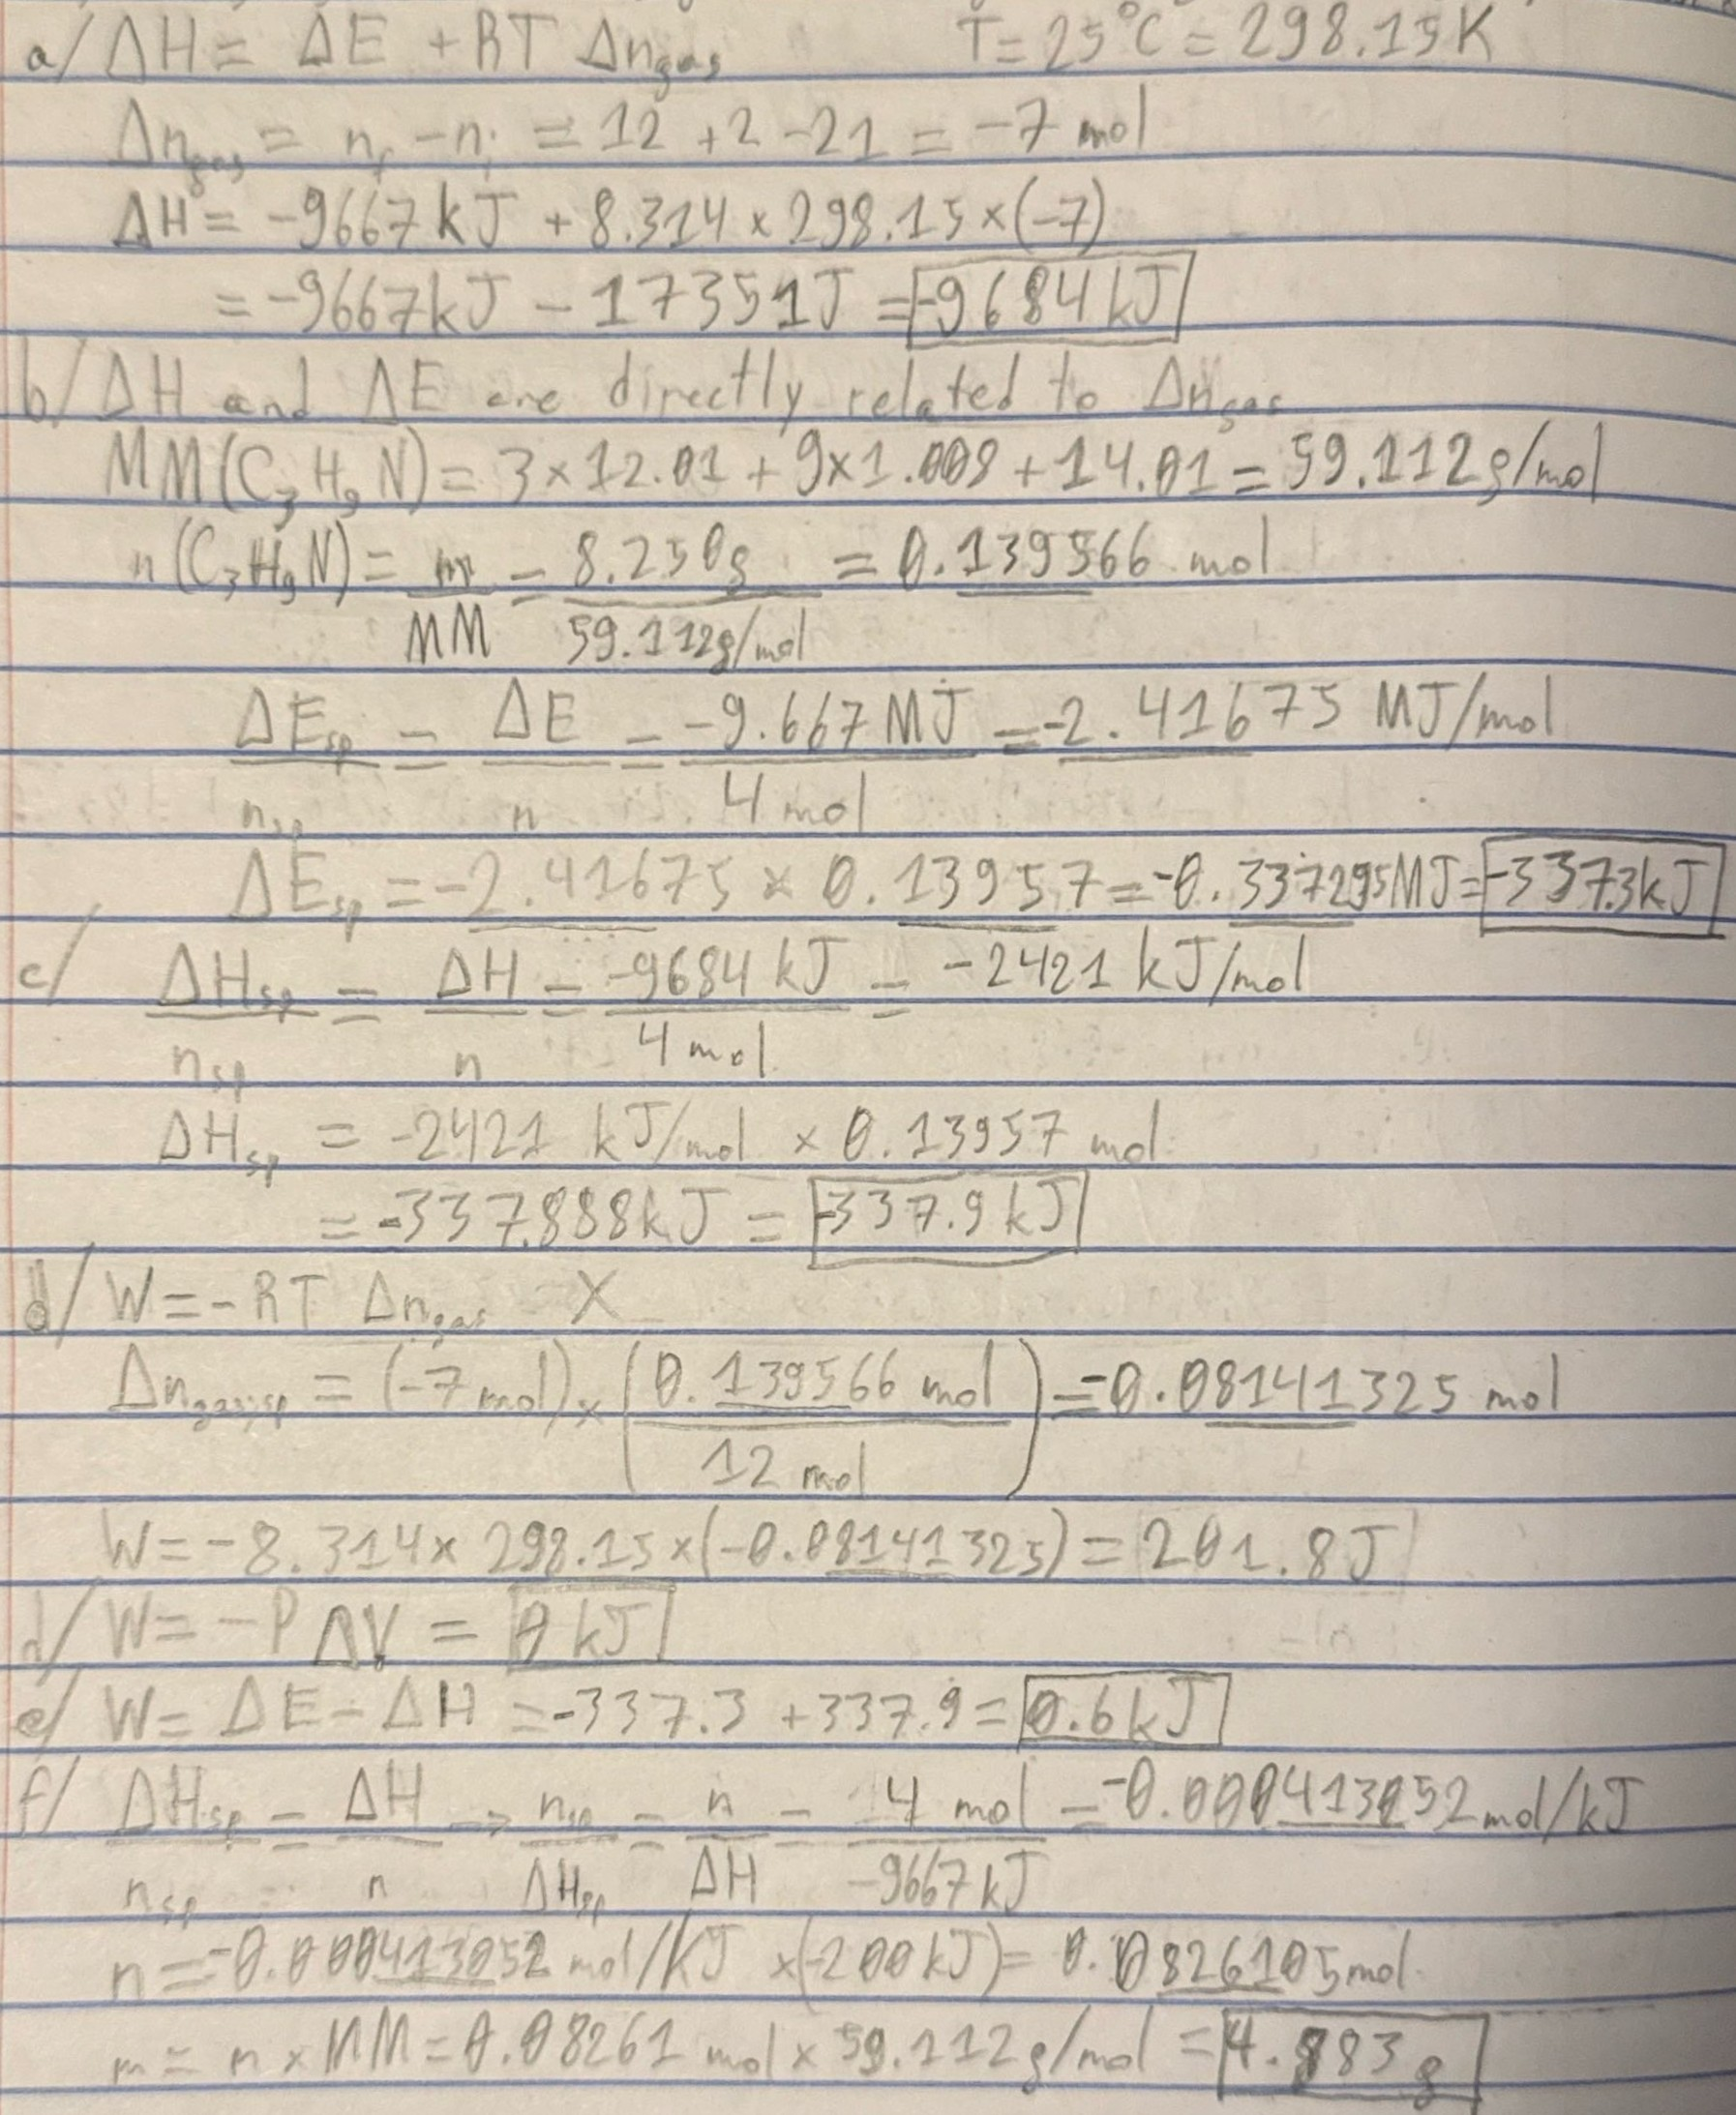
\includegraphics[width=\textwidth]{Answers Images/Problem 19 1.jpg}\\
                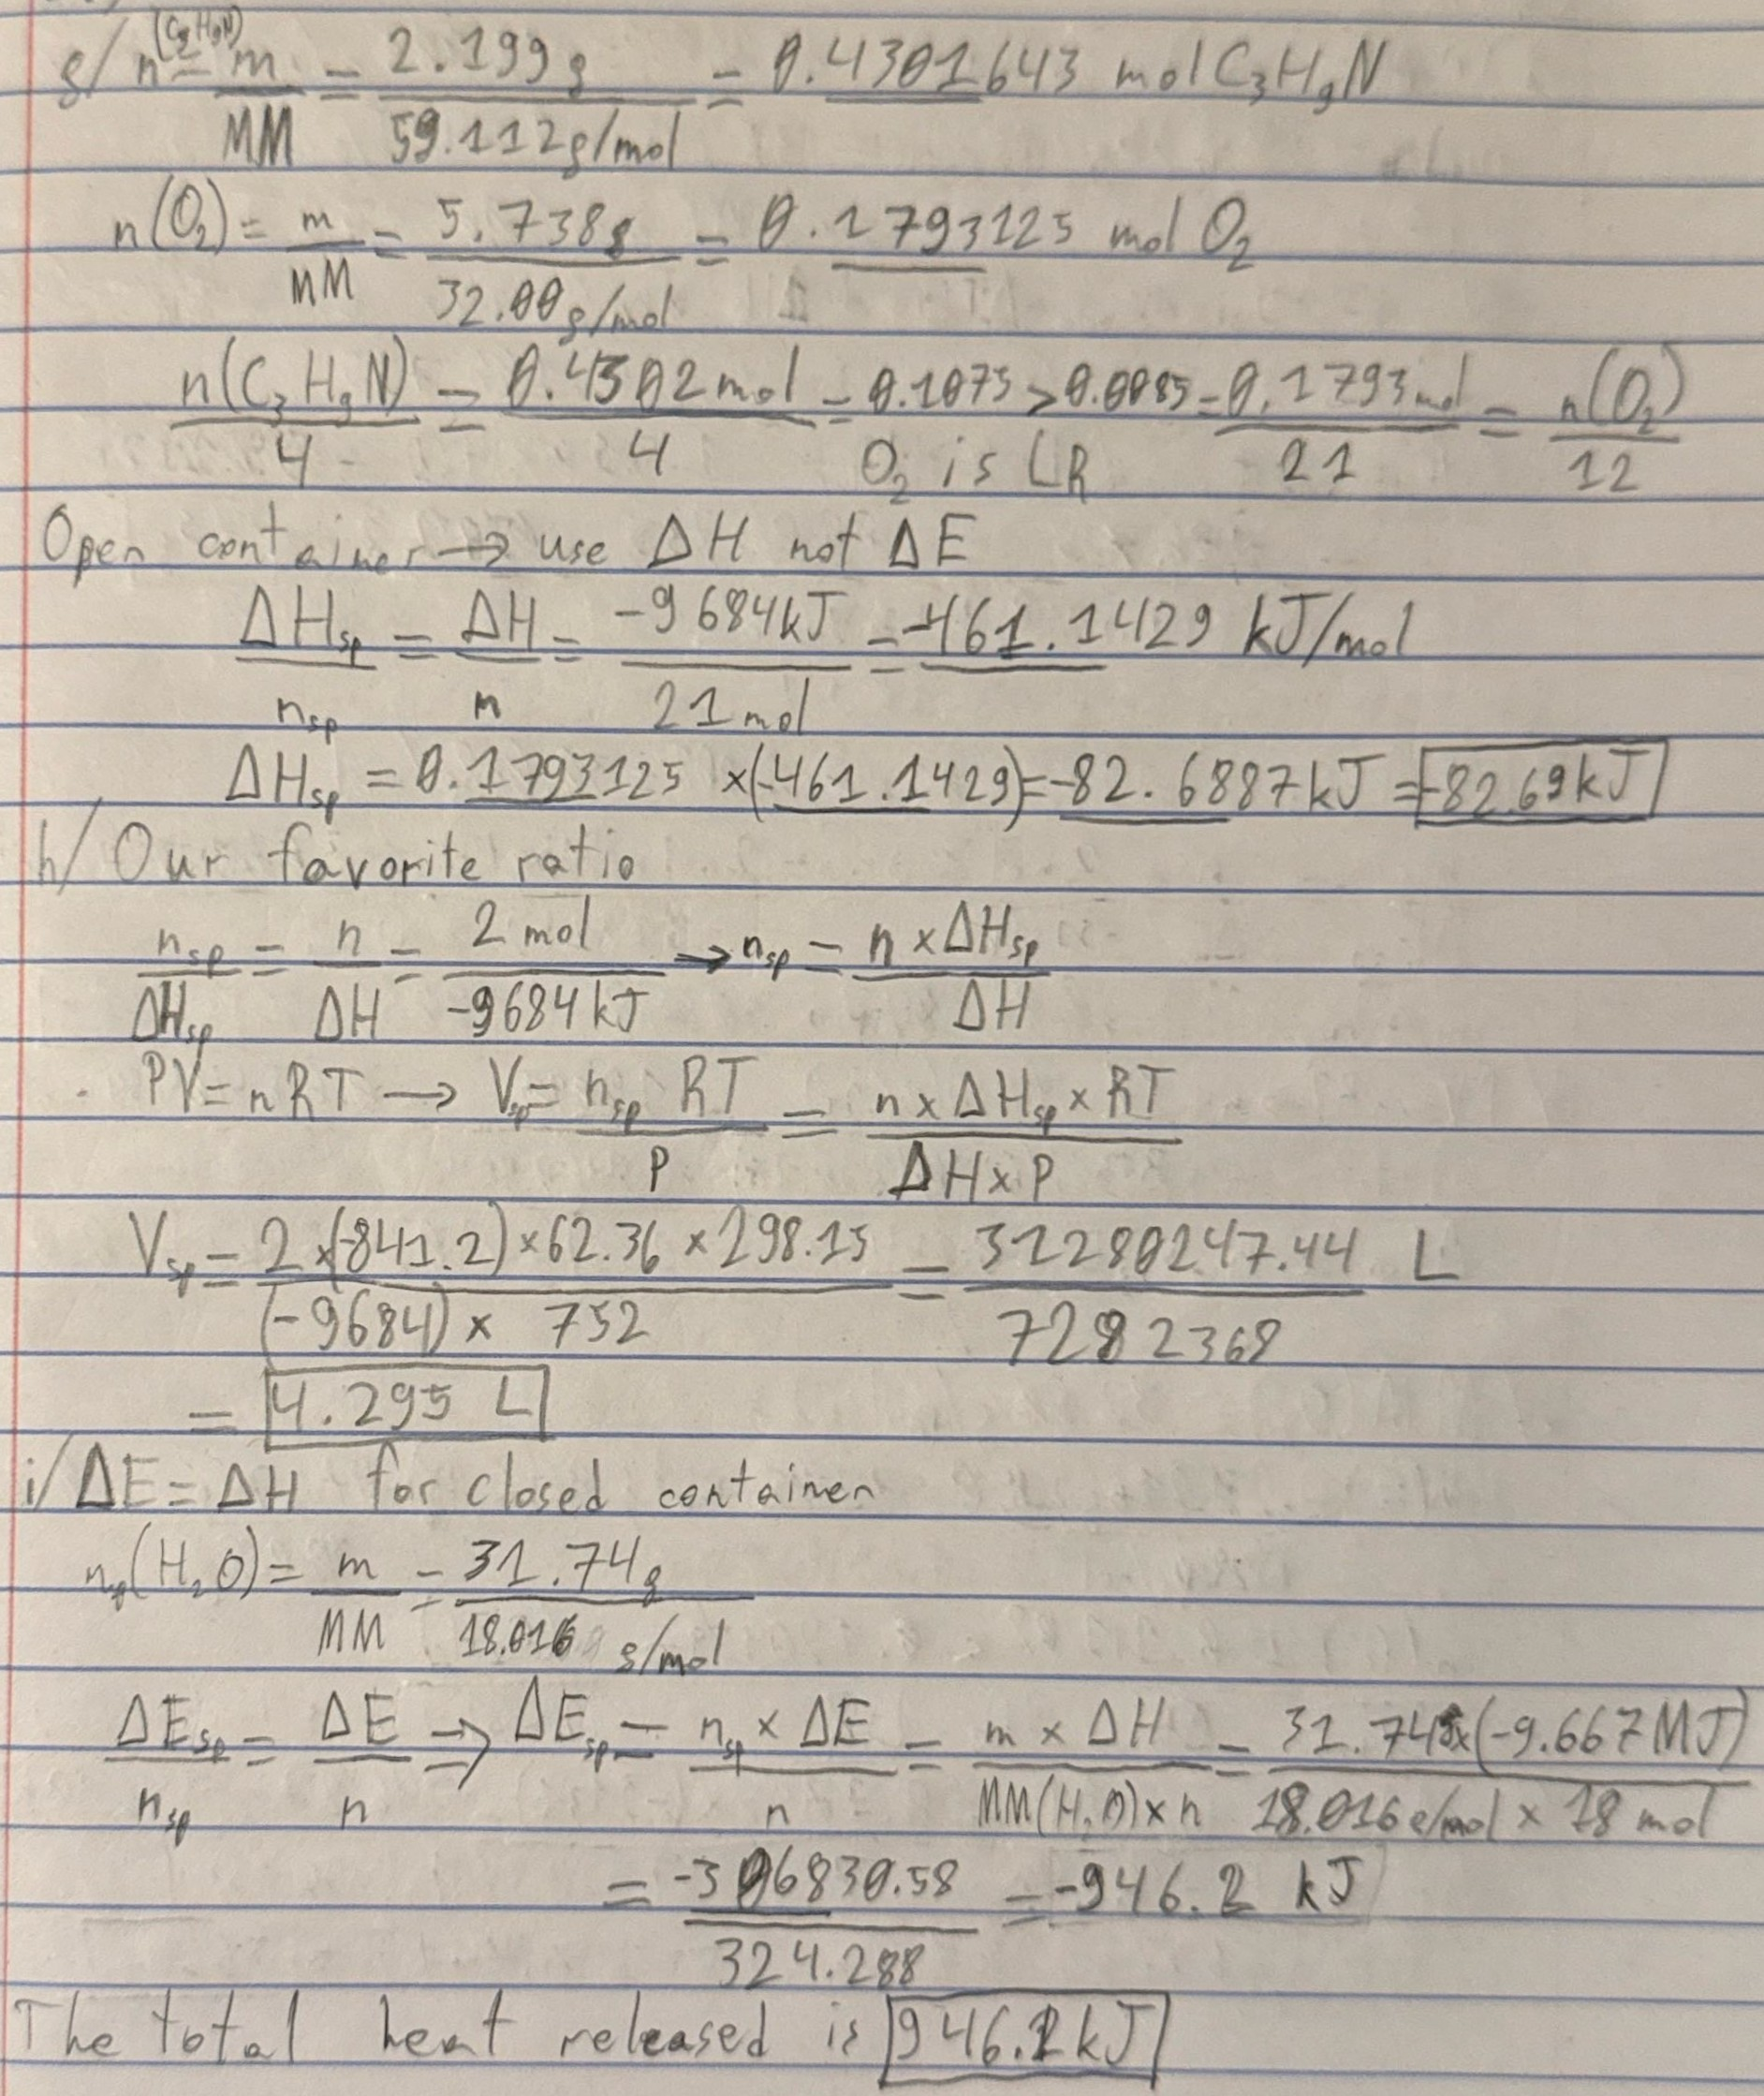
\includegraphics[width=\textwidth]{Answers Images/Problem 19 2.jpg}
            \end{center}

    \pagebreak
    \section{Topic D Problem 20}
        When 2.810 g of solid Al reacts with excess gaseous \ce{F2} in an open container at 25\unit{\celsius}, 157.3 kJ of heat is produced.
        \begin{enumerate}
            \item   Calculate $\Delta H$ and $\Delta E$ for the following reaction at 25\unit{\celsius}:\\ \ce{2 Al(s) + 3 F2(g) -> 2 AlF3(s)}
            \item   How much heat will be produced if 8.493 g of solid Al reacts with 16.610 g of gaseous \ce{F2} in a closed, rigid container at 25\unit{\celsius}? 
                Use your answer from part a to solve this problem.
        \end{enumerate}
        
        \subsection{Solution}
            \begin{center}
                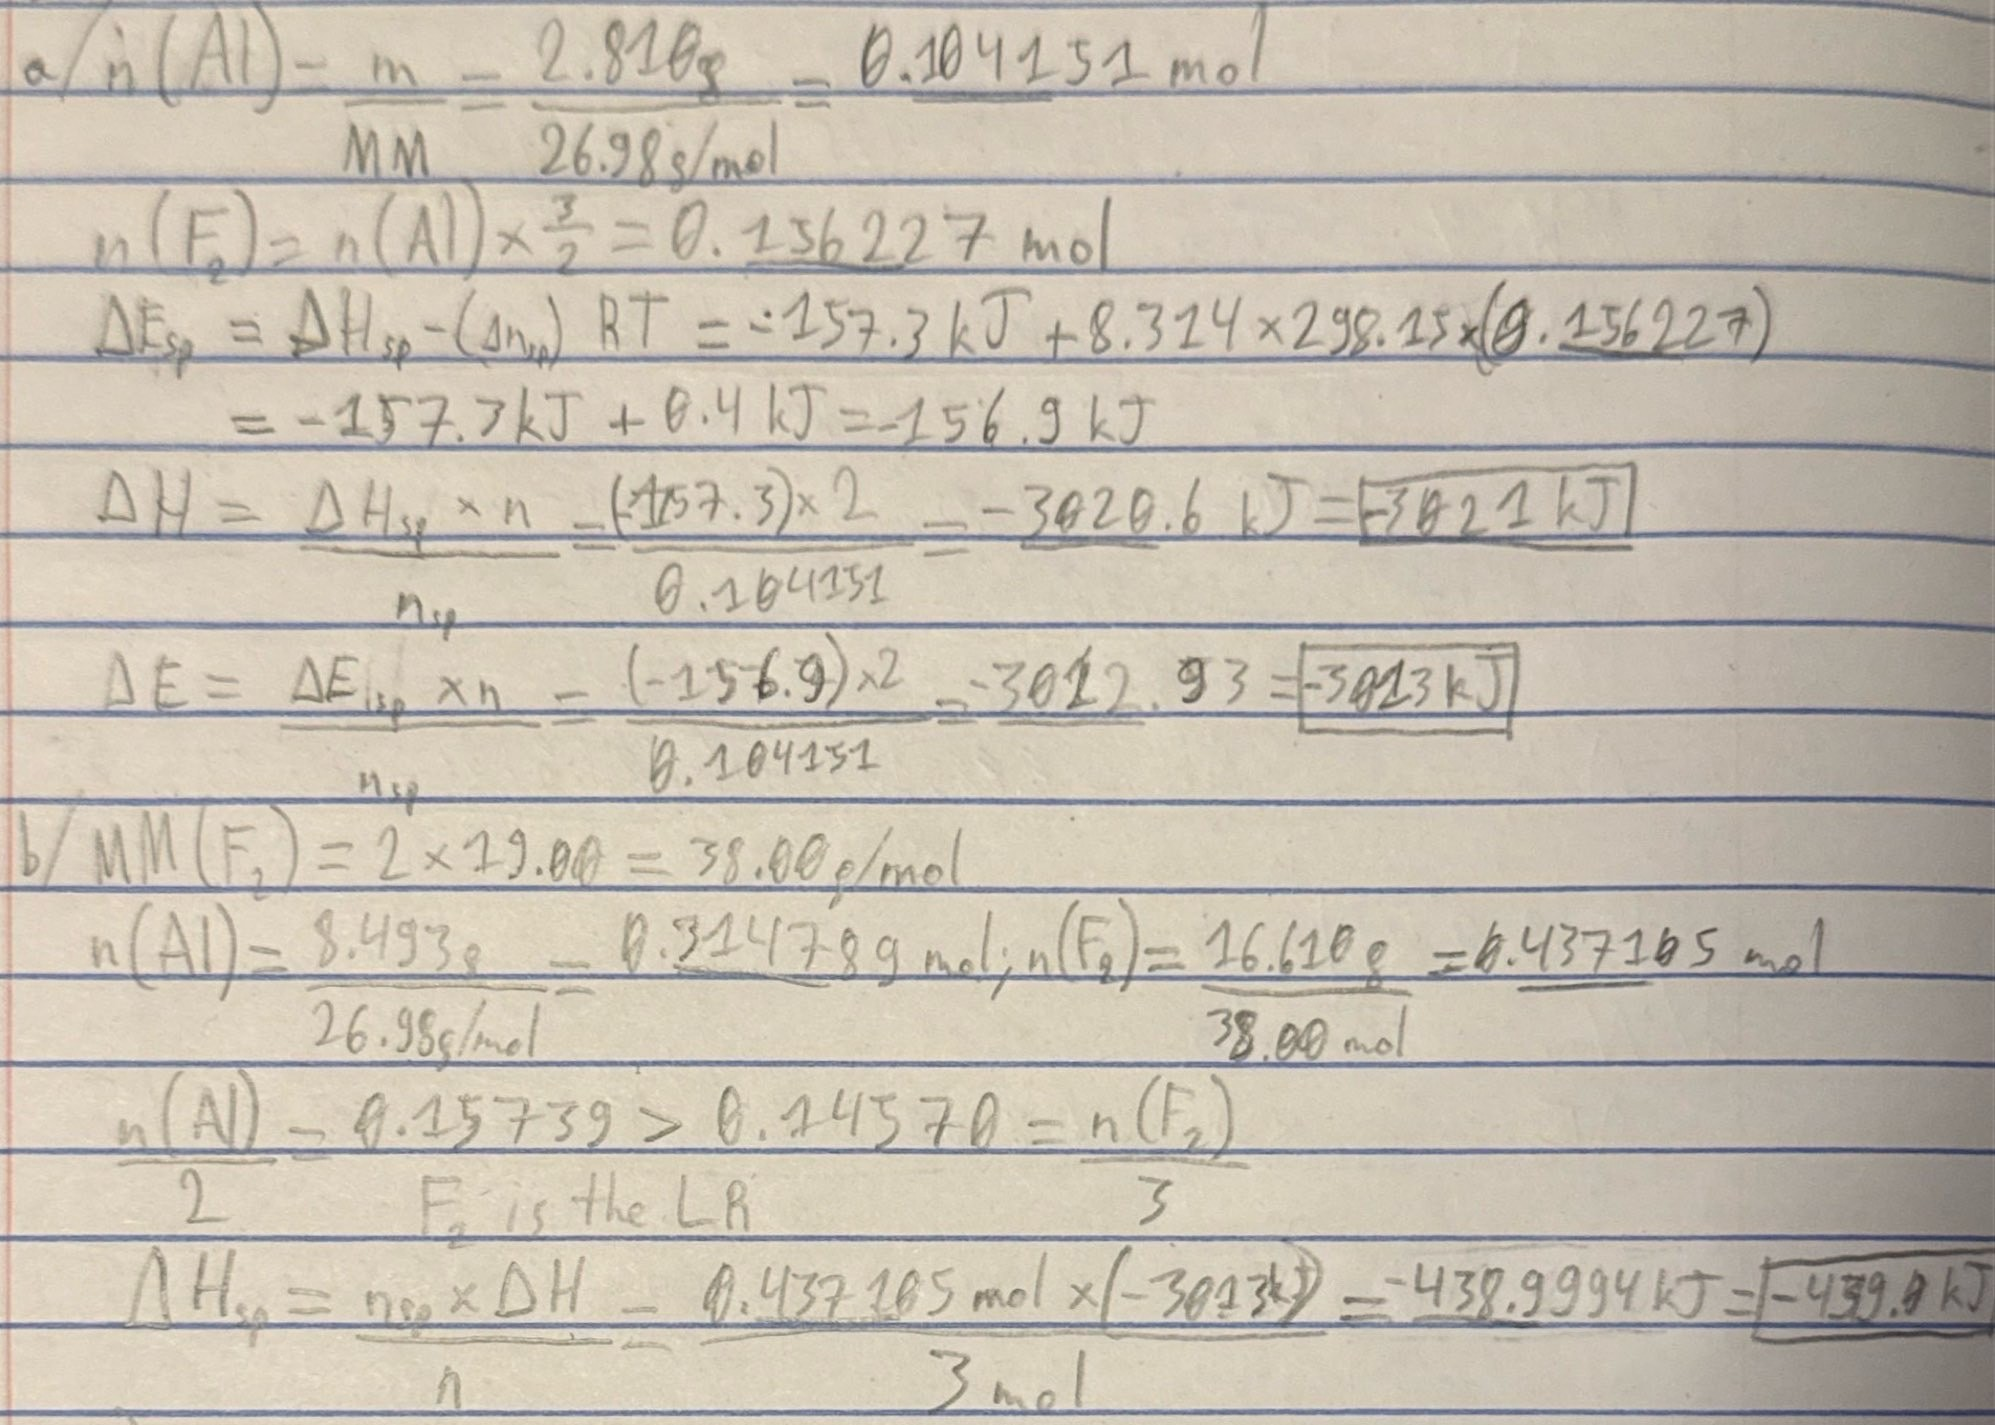
\includegraphics[width=\textwidth]{Answers Images/Problem 20.jpg}
            \end{center}

    \pagebreak
    \section{Topic D Problem 21}
        A chemist burns 1.628 g of liquid isopropyl alcohol (\ce{C3H8O}) in a bomb calorimeter that has a heat capacity of 3927 J/\unit{\celsius}. 
        The temperature of the calorimeter rises from 19.085\unit{\celsius} to 31.683\unit{\celsius} during the reaction. 
        Calculate $\Delta H$ and $\Delta E$ for the following reaction at 25\unit{\celsius}:\\
        \ce{2 C3H8O(l) + 9 O2(g) -> 6 CO2(g) + 8 H2O(l)}
        
        \subsection{Solution}
            \begin{center}
                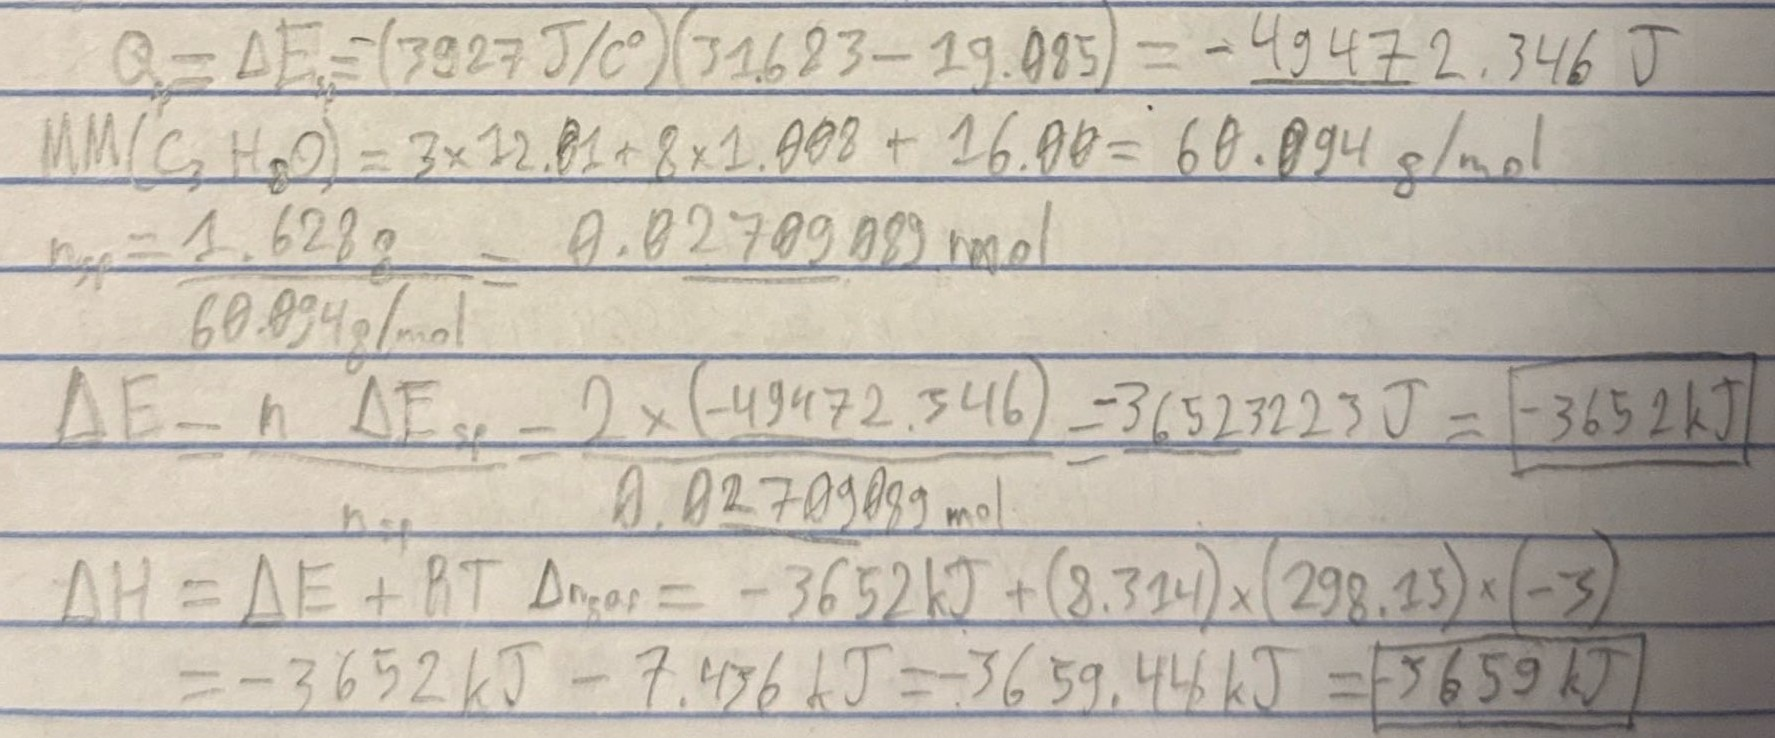
\includegraphics[width=\textwidth]{Answers Images/Problem 21.jpg}
            \end{center}

    \pagebreak
    \section{Topic D Problem 22}
        For the reaction \ce{2 C(s) + O2(g) -> 2 CO(g)}, $\Delta E$ = -219 kJ. When will $\Delta H$ also be -219 kJ?\\
        a) When the reaction is carried out in an open container.\\
        b) When the reaction is carried out in a closed, rigid container.\\
        c) $\Delta H$ will always equal $\Delta E$.\\
        d) $\Delta H$ will never equal $\Delta E$.
        
        \subsection{Solution}
            There is a constant value of $\Delta H$.
            \begin{equation}
                \rm
                \Delta H    =   \Delta E + RT \Delta n_{gas}
            \end{equation}

            Since $\rm \Delta n_{gas} = 1\,\unit{\mole}$ regardless of the conditions of the reactions, $\rm \Delta H$ will never be equal to $\rm \Delta E$.
            The only thing that will differ based on the consdition is whch wone you should use.
            For constant volume, you should use $\rm \Delta E$, while for constant pressure you should use $\rm \Delta H$.
            The answer is \boxed{(d)}. 
    
    \pagebreak
    \tableofcontents
\end{document}